\documentclass[a4paper,12pt]{article}
\usepackage[top=1in,bottom=1in,left=1in,right=1in]{geometry}
\usepackage[T1]{fontenc}
\usepackage[utf8]{inputenc}
\usepackage{lmodern}
\usepackage{textgreek}
\usepackage{amsmath}
\usepackage{mathtools}
\usepackage{graphicx}
\usepackage{svg}
\usepackage{pdflscape}
\usepackage{float}

\usepackage{tabularx}
\usepackage{blindtext}
\usepackage{hyperref}
\usepackage{pgfgantt}
\usepackage{colortbl}
\usepackage{pdfpages}
\usepackage{setspace}
\usepackage{subcaption}

\usepackage{chngcntr}
\counterwithin{figure}{subsection}
\usepackage{multicol} 


\setcounter{tocdepth}{3}
\begin{document}
	\begin{titlepage}
		\includegraphics[width=\linewidth]{graphics/ucl-banner-dl-port-outline.eps}\\[1cm]
		\center
		\setstretch{1.5}
		{ \huge \bfseries A BEng Project Interim Report}\\[1cm]
		\setstretch{1.0}

		
		\begin{multicols}{3}
			
		\Large \emph{Author:}\\
		Minduagas \textsc{Jarmolovicius}\\
		\href{mailto:zceemja@ucl.ac.uk}{zceemja@ucl.ac.uk}\\
		
		\columnbreak
		
		\Large \emph{Supervisor:}\\
		Prof. Robert \textsc{Killey}\\
		\href{mailto:r.killey@ucl.ac.uk}{r.killey@ucl.ac.uk}
		
		\columnbreak
		
		\Large \emph{Second Assessor:}\\
		Dr. Ed \\\textsc{Romans}\\
		\href{mailto:e.romans@ucl.ac.uk}{e.romans@ucl.ac.uk}
		
		\end{multicols}

		\textsc{\large Dept. of Electronic and Electrical Engineering}\\
		\textsc{\Large University College London}\\
		
		\vfill
		{\large December 13, 2019}\\[2cm]
		
	\end{titlepage}
\pagebreak

\begin{multicols}{2}

\section{Abstract}
This is abstract.
\section{Introduction}
Designed RISC has single-cycle datapath with 8bit data bus and 4 general purpose registers.

\section{The Work Performed to Date}

\subsection{Project Scheduling}
In this section present your Gantt Chart showing time management. Describe it. Be sure to distinguish term 1 work from term 2 work. Identify the dates of Progress Reports, the Viva, and the due date of the Final Project Report

\subsection{Supporting Theory}
This section outlines the theory supporting your work. Presumably you have a question that needs to be answered or a problem that needs to be solved. You may have a postulate you are trying to confirm. Whatever it might be, there is some sort of theory underlying it, otherwise you can make no deductions. Without deductions, you cannot identify needed work. Explain this to the readers.
In this section the theory 


Figure \ref{fig:simple_blocks} represents simplified diagrams of RISC and OISC architectures. In RISC architecture, program data travels from program memory to control block where instruction is decoded and further decided where what data is directed. Such structure requires complicated control block and additional data routing blocks. In order to increase performance of such processor one would need to add pipelining or add multiple cores. Both methods bring big disadvantages - multicore processor requires software adjustments and each core doubles the control and datapath substantially increasing die area; pipelinig allow operation at higher frequencies however it brings design complications such as complicated hazard prevention logic and instruction lookup. Simplicity of OISC architecture overcomes these disadvantages by following:
Pipelining can be done by individual blocks and programmibly waiting for results, multicore can be simulated by adding more data and instruction buses, hazards can be prevented with software or/and integrated into address registers. 
In addition, ALU and any other processor component can be divided by adding different address registers thus allowing to utilise multiple components at the same time given that multiple data buses are used. 

\begin{figure*}
	\centering
	\begin{subfigure}[b]{1\textwidth}
		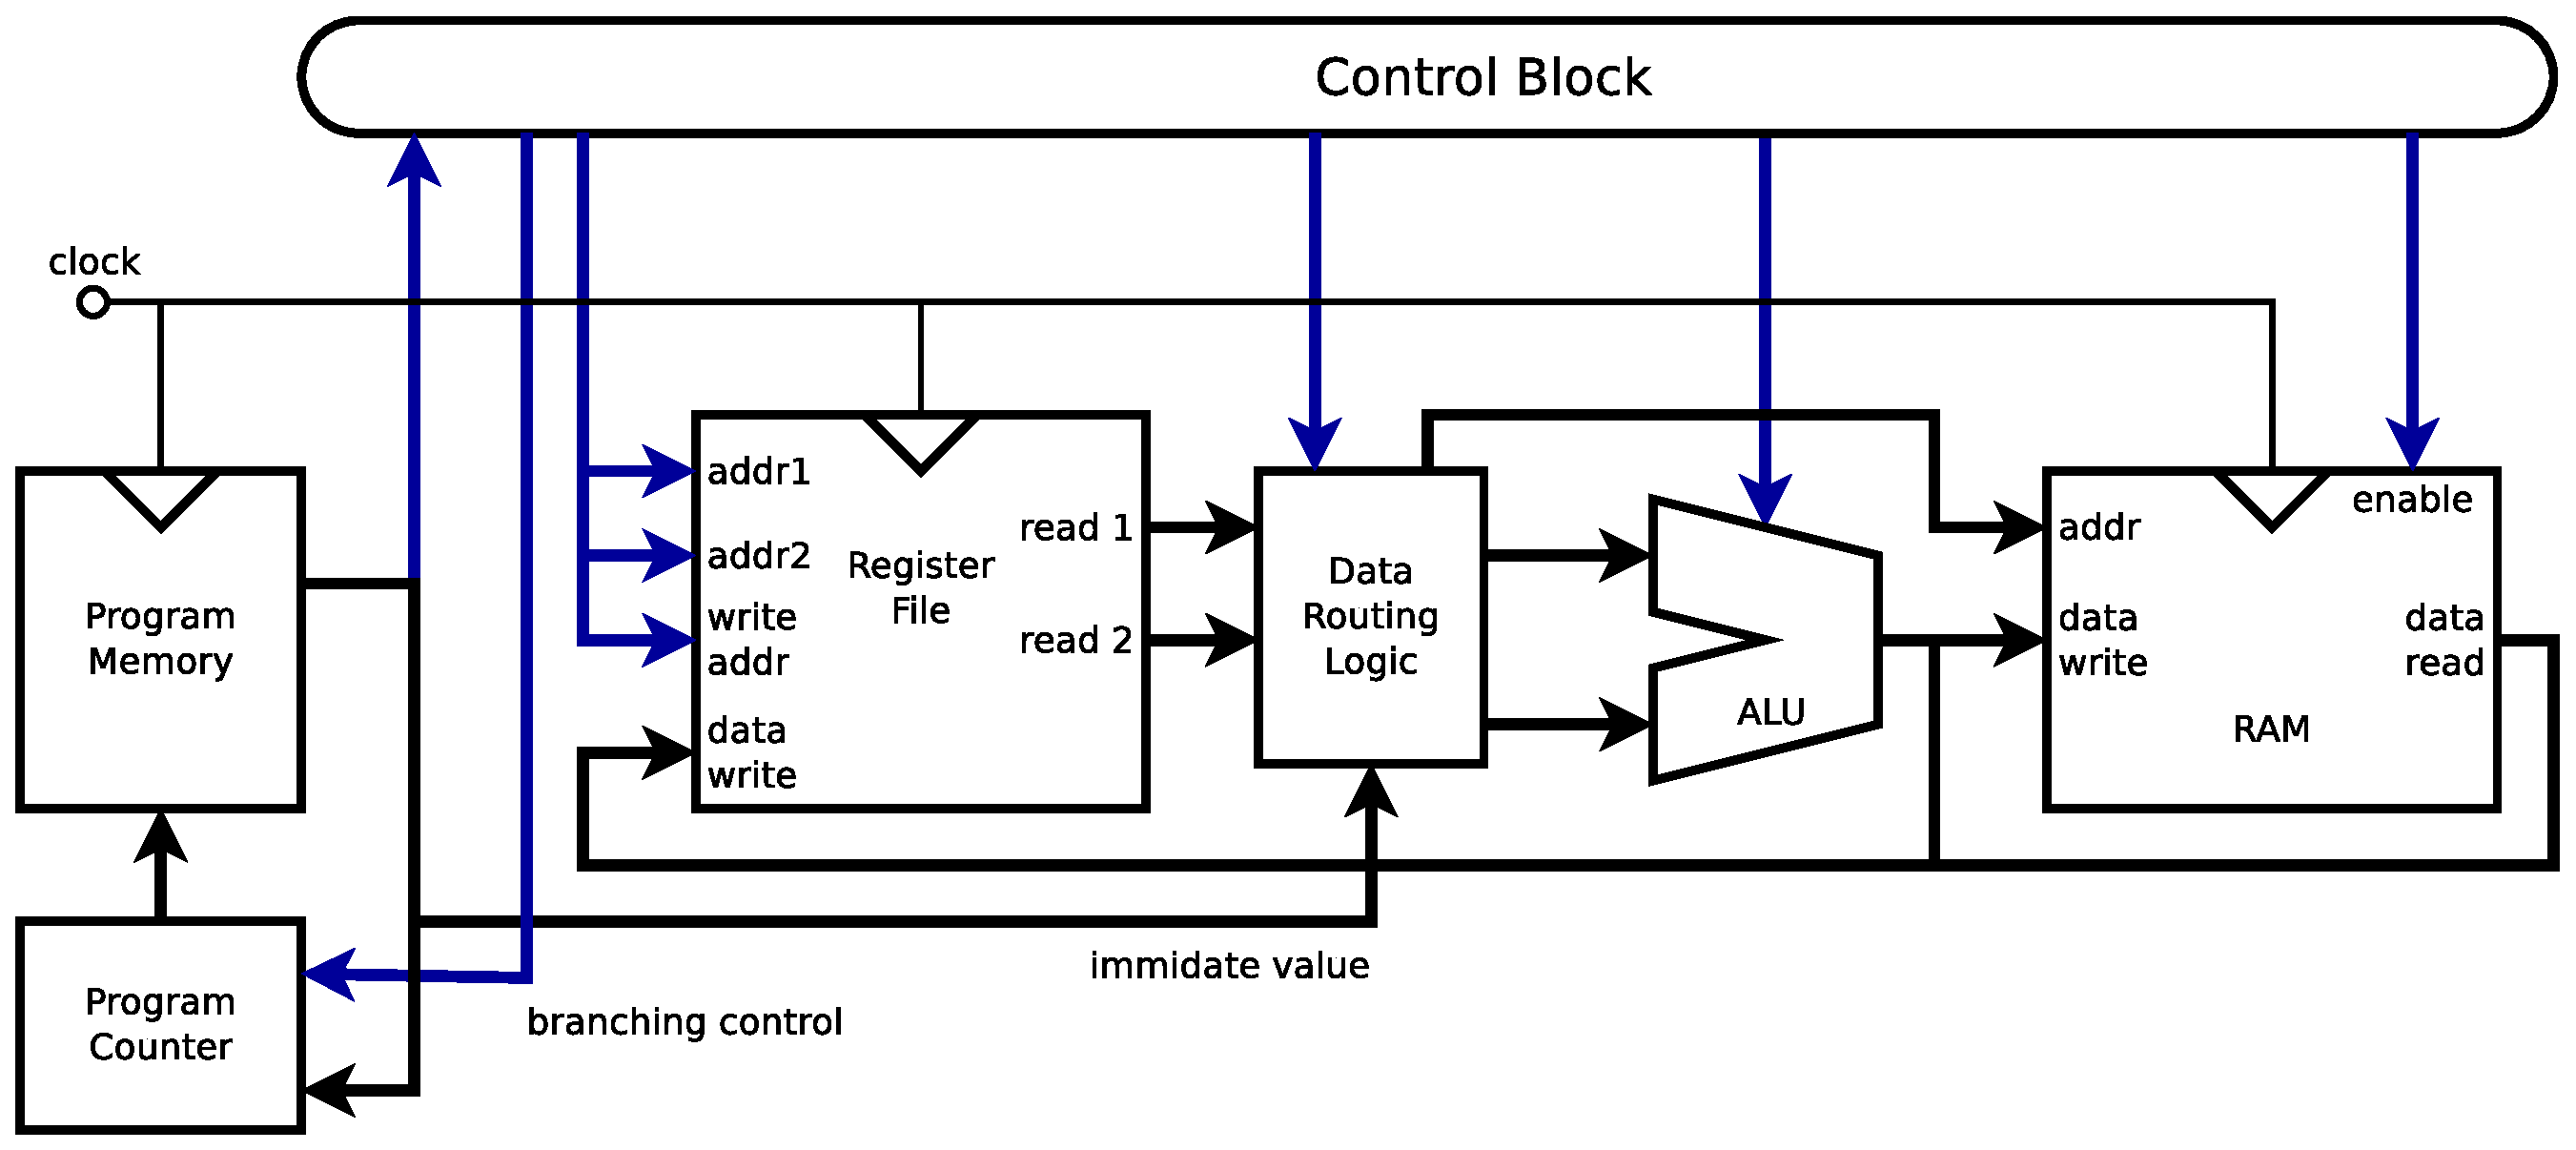
\includegraphics[width=\linewidth]{graphics/risc.eps}
		\caption{RISC microarchitecture}
		\label{fig:risc_simple}
	\end{subfigure}
	
	\begin{subfigure}[b]{1\textwidth}
		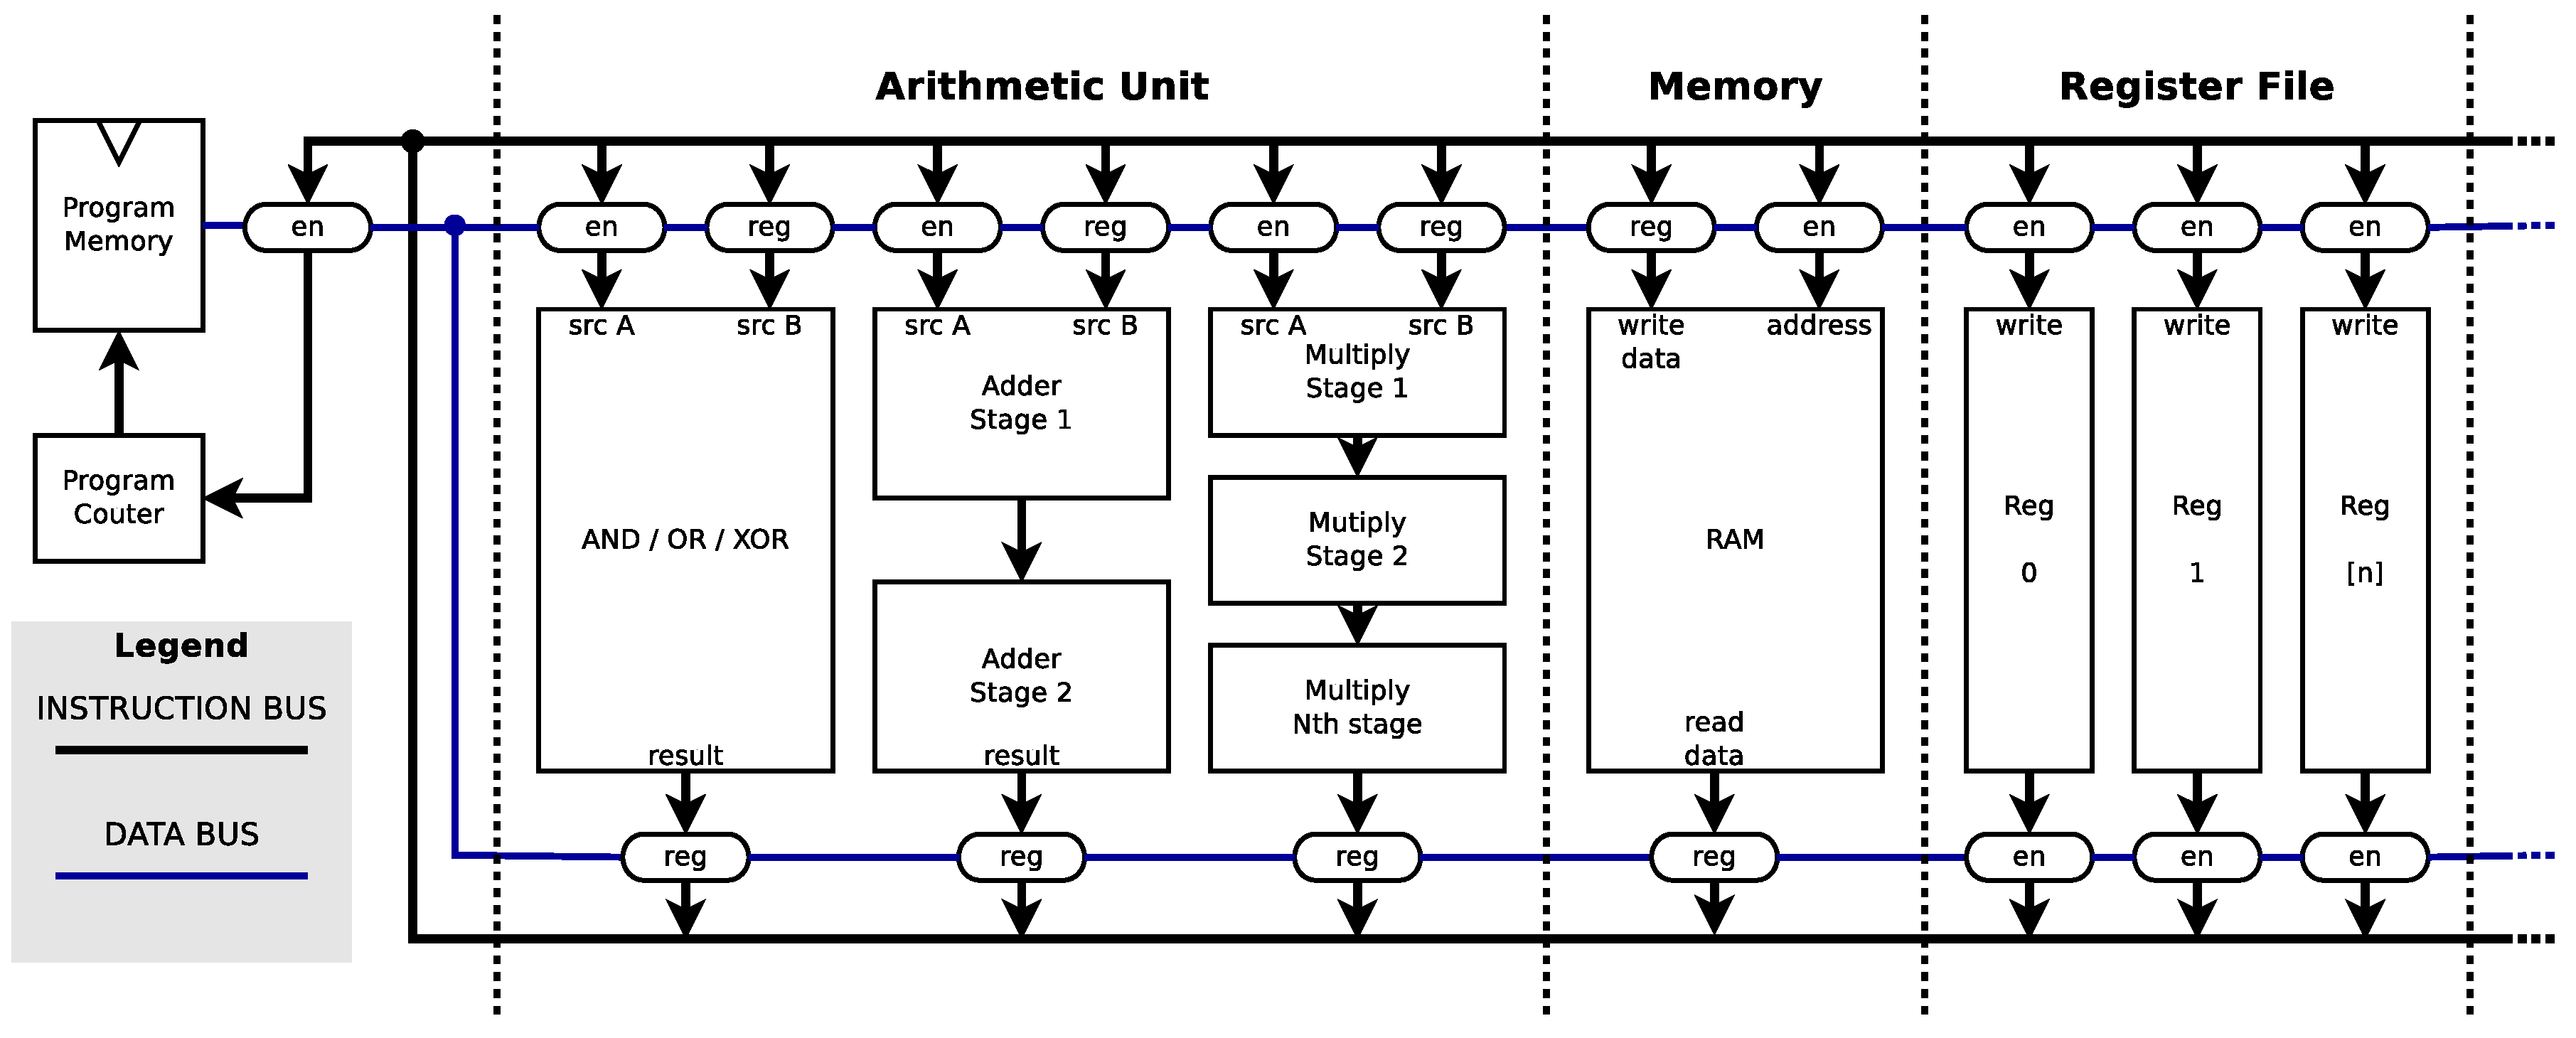
\includegraphics[width=\linewidth]{graphics/oisc.eps}
		\caption{Single data bus OISC microarchitecture}
		\label{fig:oisc_simple}
	\end{subfigure}
	
	\caption{Simplified diagrams of both architectures. Blue lines indicate control/instruction buses and black - data buses}
	\label{fig:simple_blocks}
\end{figure*}

\subsection{Progress to Date}
Use as many sections as you need to in order to discuss your progress so far. For example, you can use a different section to discuss each bit of the system to be constructed or designed.Include difficulties and issues impeding progress.

\subsubsection{Program Counter}
\begin{figure*}
	\centering
	\includegraphics[width=\linewidth]{graphics/program_counter.eps}
	\caption{Digital diagram of RISC8 program counter}
\end{figure*}


\subsubsection{Stack Pointer}

\section{Summary of Difficulties and Issues}
This chapter focuses on any difficulties or issues that are hindering you from moving forward or are slowing you down. Your Supervisor needs to know whether other coursework is keeping you from progressing more rapidly or if parts are not arriving as expected, or if something else is bothering you. You may have made notes of these already in Chapter 2, but now is the time to bring them together and summarise them for your Supervisor.


\subsection{List of Difficulties}
Use a bullet list and then explain each one in more detail. You may also refer back to sections in Chapter 2
\begin{description}
	\item[$\bullet$] Assembler - writing a flexible code that would convert assembly code with labels, sections and macros to machine code;
	\item[$\bullet$] Memory - trying to develop easy to use ROM and RAM memory;
	\item[$\bullet$] Timing - problems with multiple components in datapath due to RAM and ROM registers;
	\item[$\bullet$] JTAG - issues with JTAG interface that communicates with FPGA.
\end{description}

\subsubsection{Assembler}
\subsubsection{Memory}
Initial plan was to use 32MBit 16-bit data width, SDRAM chip located at FPGA board. After successfully simulating most of processor functions, next step was to synthesise and run it on FPGA which brought 2 problems:

1. Uploading program into ROM is not simple as generic Verilog unpacked register array cannot be initialised from file. This problem was solved by using FPGA built-in M9K memory that allows flexible RAM/ROM configuration. In addition, this memory can be read from/written to via JTAG connection without affecting FPGA operation. This also enabled quick method to upload programs without need to resynthesising processor code;

2. Timing problems with SDRAM memory controller as it runs at higher frequency than processor (at 100MHz versus 1MHz), used interface between them was multiple 1-word length FIFO registers which caused memory read operation take 2 processor cycles. 3 possible solutions were considered - suspend processor clock while memory data is read, remove FIFO registers and rely on SDRAM clock being much greater than processor clock, use M9K. Last option was chosen due to ease of implementation and ability to read RAM content via JTAG for debugging purposes.
\subsubsection{Timing}

\subsubsection{Return instruction}

\subsubsection{JTAG}
At multiple occasions FPGA could not be controlled due to JTAG error code that indicated that there is problem with commutation between JTAG controller on the board and the rest of a chain. After long investigation it was concluded that this problem is caused by Linux JTAG Daemon service that needs to be simply restarted. 

\subsection{Failure Assessment}
Focus on the possibility of failure in this section and assessthe likelihood ofthe most important steps of the project not reaching a conclusion. Identify all those things that must come together in order for the project to be successful and discover which are the most likely to fail and by what measure. Identify mitigation procedures.

\subsection{Updated Safety Risk Assessment}
There are no changes to Safety Risk Assessment.

\end{multicols}

\newpage
\begin{landscape}
	\section{Updated Schedule}
	\begin{table}[h]
		\centering
		\begin{ganttchart}[
			y unit title=0.4cm,
			y unit chart=0.5cm,
			x unit=1.1mm,
			hgrid,
			today=2019-12-13,
			today label node/.append style={below=12pt},
			today label font=\itshape\color{blue},
			today rule/.style={draw=blue, ultra thick},
			title height=1,
			bar/.append style={fill=blue!50},
			bar incomplete/.append style={fill=gray!50},
			progress label text={$\displaystyle{#1\%}$},
			time slot format=isodate
			]{2019-10-01}{2020-03-31}
			\gantttitlecalendar{year, month=shortname} \\
			\gantttitle{40}{6}
			\gantttitlelist{41,...,52}{7}
			\gantttitlelist{1,...,13}{7}
			\gantttitle{}{2} \\
			\ganttbar[progress=100]{RISC implementation}{2019-10-01}{2019-10-27}\\
			\ganttbar[progress=90]{RISC Optimisations}{2019-10-27}{2019-11-25}\\
			\ganttbar[progress=100]{UART and I/O}{2019-10-21}{2019-10-27}
			\ganttbar[progress=100]{}{2019-11-25}{2019-12-08} \\
			\ganttbar[progress=100]{RISC Assembler}{2019-10-14}{2019-11-11}\\
			\ganttbar[progress=20]{Developing benchmark}{2019-11-11}{2019-12-13}
			\ganttbar[progress=0]{}{2020-02-23}{2020-03-07} \\
			\ganttbar[progress=10]{OISC Implementation}{2019-12-02}{2019-12-13}
			\ganttbar[progress=0]{}{2020-01-13}{2020-02-02}\\
			\ganttbar[progress=0]{OISC Optimisations}{2020-02-02}{2020-02-23}\\
			\ganttbar[progress=0]{OISC Assembler}{2020-01-20}{2020-02-09}\\
			\ganttbar[progress=0]{OISC Compiler}{2020-02-09}{2020-03-01}\\
			\ganttmilestone{Project Proposal finalised}{2019-10-14}\\
			\ganttmilestone{Progress Report \#1}{2019-11-04}\\
			\ganttmilestone{Progress Report \#2}{2019-11-25}\\
			\ganttmilestone{December Interim Report}{2019-12-13}\\
			\ganttmilestone{Progress Report \#3}{2020-01-20}\\
			\ganttmilestone{Progress Report \#4}{2020-02-14}\\
			\ganttmilestone{Progress Report \#5}{2020-03-02}\\
			\ganttmilestone{Poster Presentation}{2020-03-18}\\
			\ganttmilestone{Final Report}{2020-03-30}\\
			\ganttvrule{Reading Week}{2019-11-03}
			\ganttvrule{}{2019-11-10}
			\ganttvrule[vrule label node/.append style={anchor=north west}]{Holidays}{2019-12-13}
			\ganttvrule{}{2020-01-12}
		\end{ganttchart}	
		\caption{Updated project schedule Grantt chart}
		\label{table:time}
	\end{table}
\end{landscape}

\section{Appendix A: Safety Risk Assessment}
Append your updated Safety Risk Assessment whether approved in RiskNet or not. This should be the page that is signed by your Supervisor and by your lab manager(s).

\section{Appendix B: Computer Code}
Append any code you may need here. Reference it in the text as "Appendix B, code snippet \#"; for example,"Finda sample of the code usedfor this experiment in Appendix B, code snippet 2".

\section{References}


\end{document}